\documentclass[a4paper, 10pt]{article}

\usepackage[default]{comfortaa}
\usepackage[utf8]{inputenc}
\usepackage[english]{babel}
\usepackage{graphicx}
\usepackage{geometry}
\usepackage{titlesec}
\usepackage{multicol}
\usepackage{lastpage}
\usepackage{fancyhdr}
\usepackage{array}
\usepackage{multirow, hhline}
\usepackage[table]{xcolor}
\usepackage[hidelinks]{hyperref}
\usepackage{textcomp}

\setlength{\columnsep}{1cm}

\definecolor{lightgray}{gray}{0.85}

\setlength{\arrayrulewidth}{0.35mm}
\setlength{\tabcolsep}{10pt}
\renewcommand{\arraystretch}{2}

\fancypagestyle{plain}{%
\fancyhf{} % clear all header and footer fields
\cfoot{\thepage /\pageref{LastPage}}
\rfoot{\href{https://github.com/ElectricCanary/Bontempo}{
\includegraphics[width=5mm, height=5mm]{github}}\hspace{8pt}\href{https://www.facebook.com/ElectricCanary}{
\includegraphics[width=5mm, height=5mm]{f}}\hspace{8pt}\href{https://www.instagram.com/electricanary/}{
\includegraphics[width=5mm, height=5mm]{inst}}\hspace{12pt}\href{mailto:support@electric-canary.com}{
\includegraphics[width=5mm, height=5mm]{email}}}
\lfoot{\textcolor{black!70}{{\footnotesize\textcopyright Electric Canary - June 2020}}}
\renewcommand{\headrulewidth}{0pt}
\renewcommand{\footrulewidth}{0pt}}


\pagestyle{fancy}
\renewcommand{\headrulewidth}{0pt}
\cfoot{}
\cfoot{\thepage /\pageref{LastPage}}
\rfoot{\href{https://github.com/ElectricCanary/Bontempo}{
\includegraphics[width=5mm, height=5mm]{github}}\hspace{8pt}\href{https://www.facebook.com/ElectricCanary}{
\includegraphics[width=5mm, height=5mm]{f}}\hspace{8pt}\href{https://www.instagram.com/electricanary/}{
\includegraphics[width=5mm, height=5mm]{inst}}\hspace{12pt}\href{mailto:support@electric-canary.com}{
\includegraphics[width=5mm, height=5mm]{email}}}
\lfoot{\textcolor{black!70}{{\footnotesize\textcopyright Electric Canary - June 2020}}}
\rhead{\href{https://electric-canary.com/bontempo}{
\includegraphics[scale=0.22]{logo}}}
\lhead{\textbf{{\small\emph{\textcolor{black!70}{Bontempo - Build Documentation}}}}}

\titleformat*{\section}{\huge\bfseries}
\titleformat*{\subsection}{\LARGE\bfseries}
\titleformat*{\subsubsection}{\Large\bfseries}

\geometry{hmargin=2.5cm,vmargin=2.5cm}
\headheight=35pt

\begin{document}\thispagestyle{plain}
\begin{center}
\begin{Huge}
\vspace*{0.5cm}
\textbf{Bontempo - Build Documentation}
\rule {0.95\textwidth}{2pt}\\
\end{Huge}
\vspace{1cm}

\includegraphics[scale=1]{logocentre}\\
\end{center}
\vspace{1cm}
Bontempo is a Tap Tempo \& Modulation solution for PT2399 delay. You do need a PT2399 delay circuit to use with the Bontempo PCB. This is a build guide for the Bontempo PCB. For any information about operating the Bontempo please refer to the \href{https://electric-canary.com/assets/bontempo---datasheet.pdf}{\underline{datasheet}}. \\

\vfill
\begin{center}
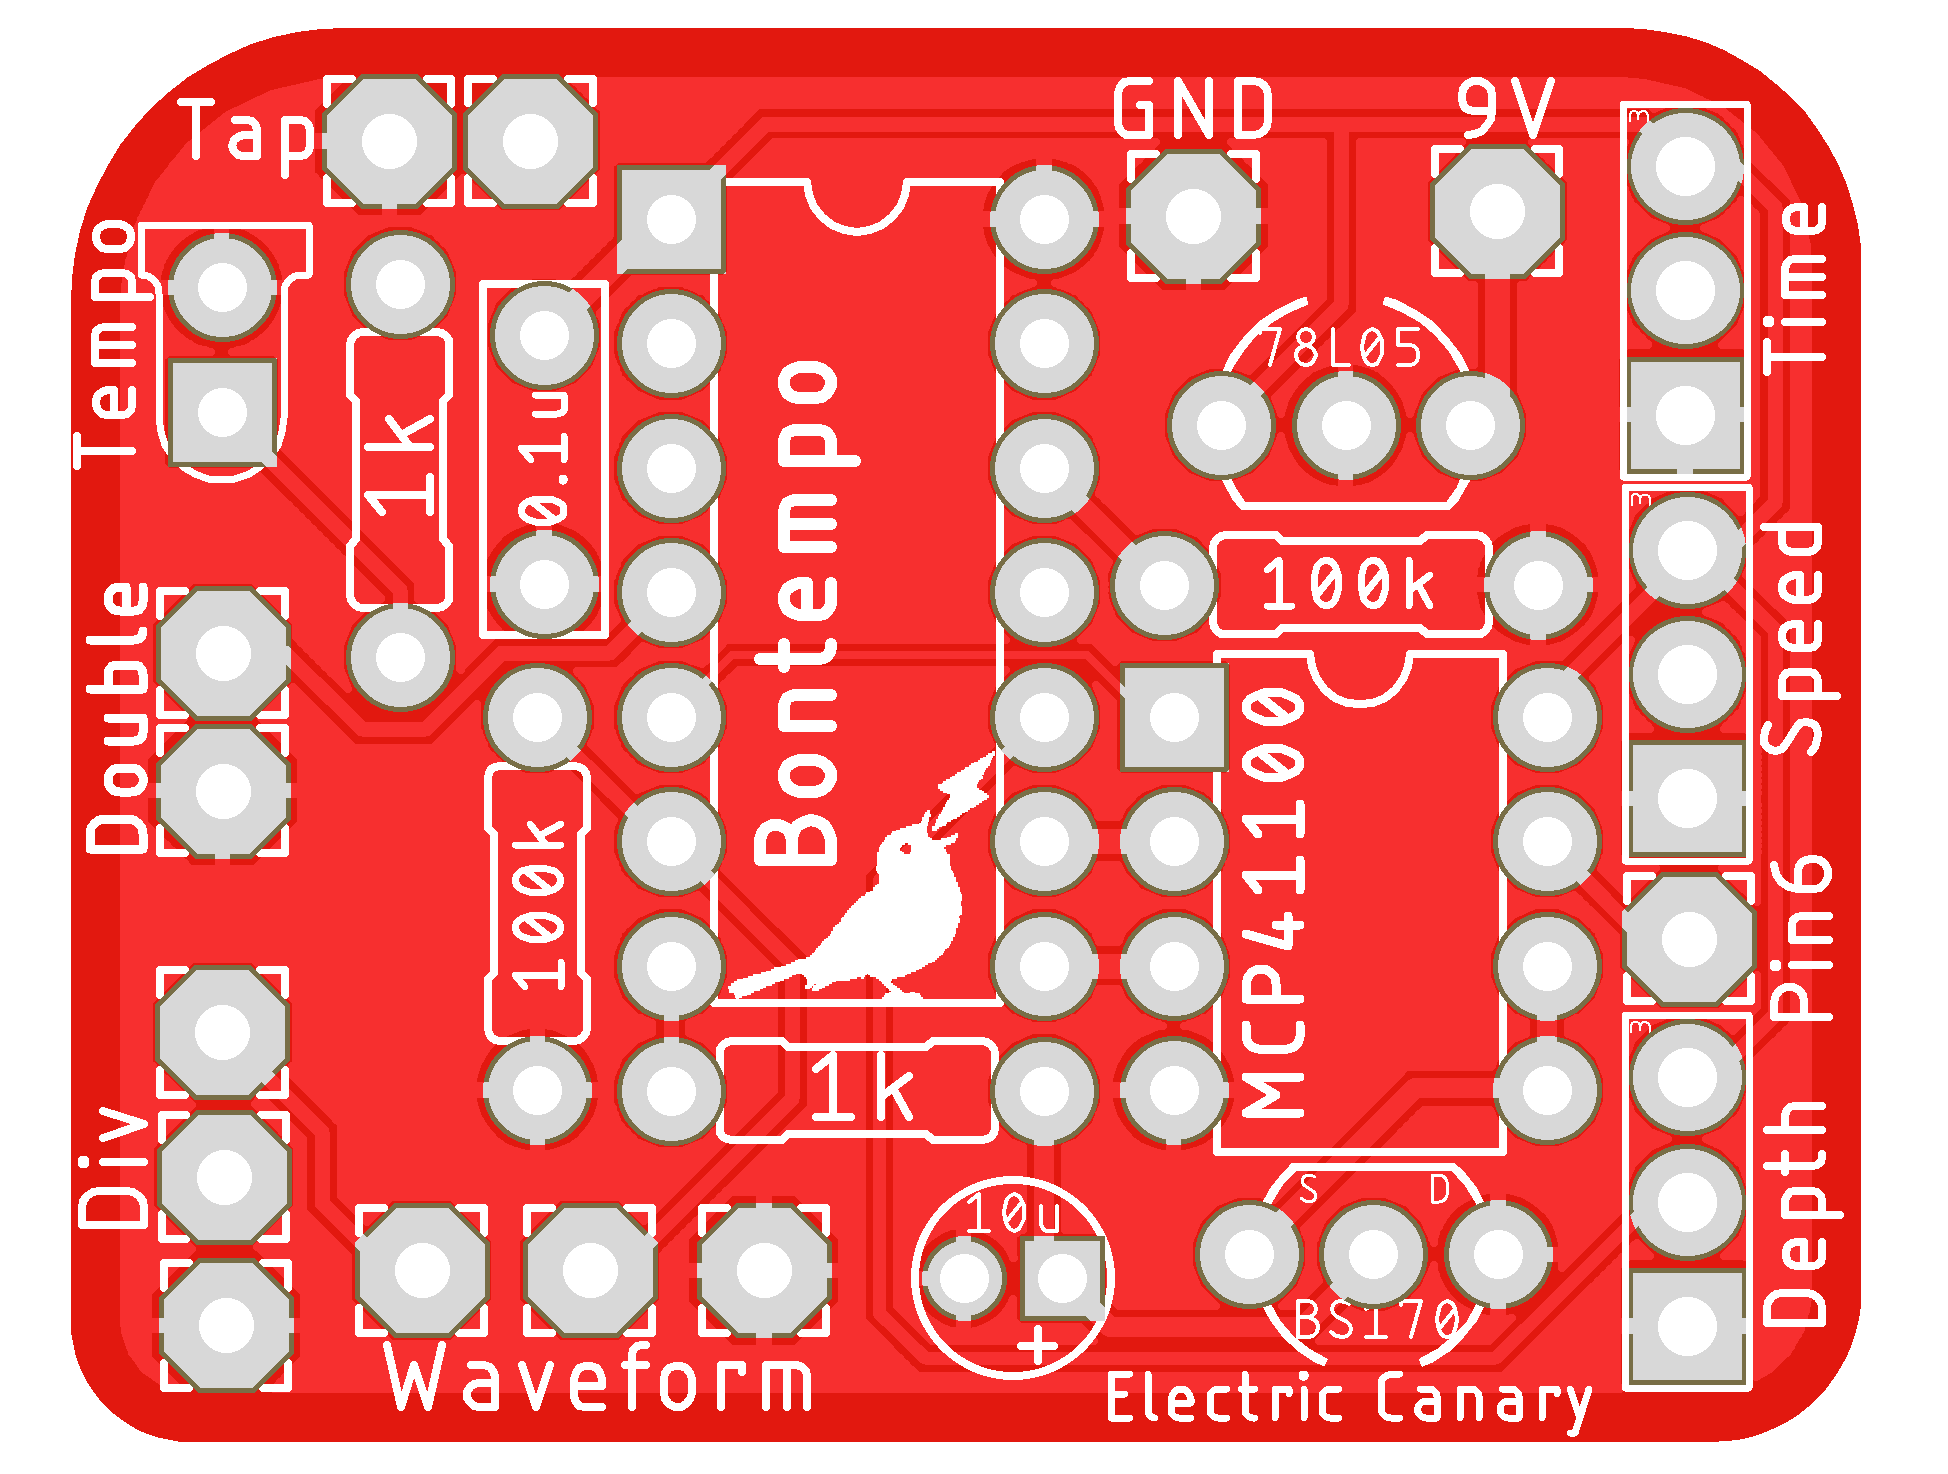
\includegraphics[scale=0.3]{BontempoPCB}
\end{center}
\vfill
\newpage
\section{Schematic}
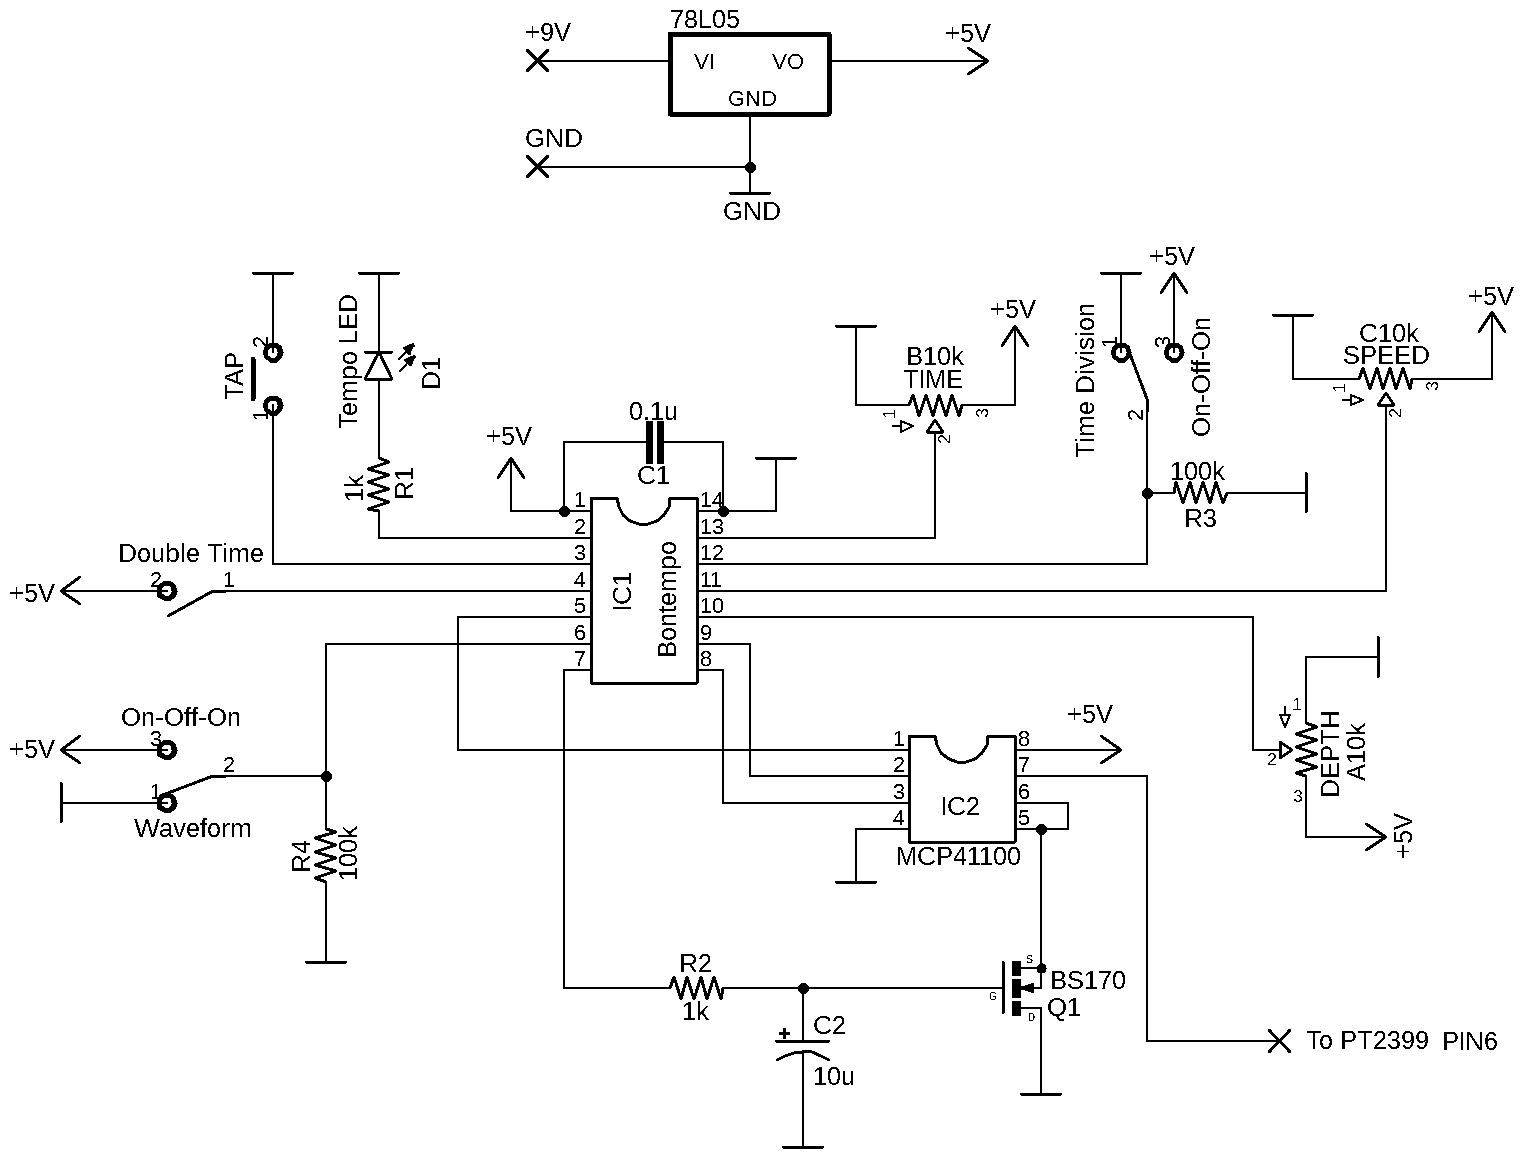
\includegraphics[scale=1.1]{Schematic}
\section{Bill of Materials}
\begin{multicols}{2}
{\rowcolors{1}{}{lightgray!50}
\begin{tabular}{|c|c|}
\hline
\rowcolor{gray}{\LARGE\textcolor{white}{\textbf{Name}}} &  {\LARGE\textcolor{white}{\textbf{Value}}}\\
\hline
R1 & 1k$\Omega$ (more for dimmer LED)\\
\hline
R2 & 1k$\Omega$ \\
\hline
R3 & 100k$\Omega$ \\
\hline
R4 & 100k$\Omega$ \\
\hline
C1 & 100nF \\
\hline
C2 & 10$\mu$F \\
\hline
 &  \\
\hline
D1 & Tempo LED \\
\hline
Q1 & BS170 \\
\hline
\end{tabular}}
\columnbreak
\begin{flushright}
{\rowcolors{1}{}{lightgray!50}
\begin{tabular}{|c|c|}
\hline
\rowcolor{gray}{\LARGE\textcolor{white}{\textbf{Name}}} &  {\LARGE\textcolor{white}{\textbf{Value}}}\\
\hline
IC1 & Bontempo\\
\hline
IC2 & MCP41100 \\
\hline
Time & B10k\\
\hline
Speed & C10k \\
\hline
Depth & A10k \\
\hline
Tap & Momentary SPST \\
\hline
Time Division & SPDT On-Off-On \\
\hline
Waveform & SPDT On-Off-On \\
\hline
Double Time & SPST \\
\hline
\end{tabular}}
\end{flushright}
\end{multicols}
\newpage
\section{Wiring Diagram}
\bigbreak
\begin{center}
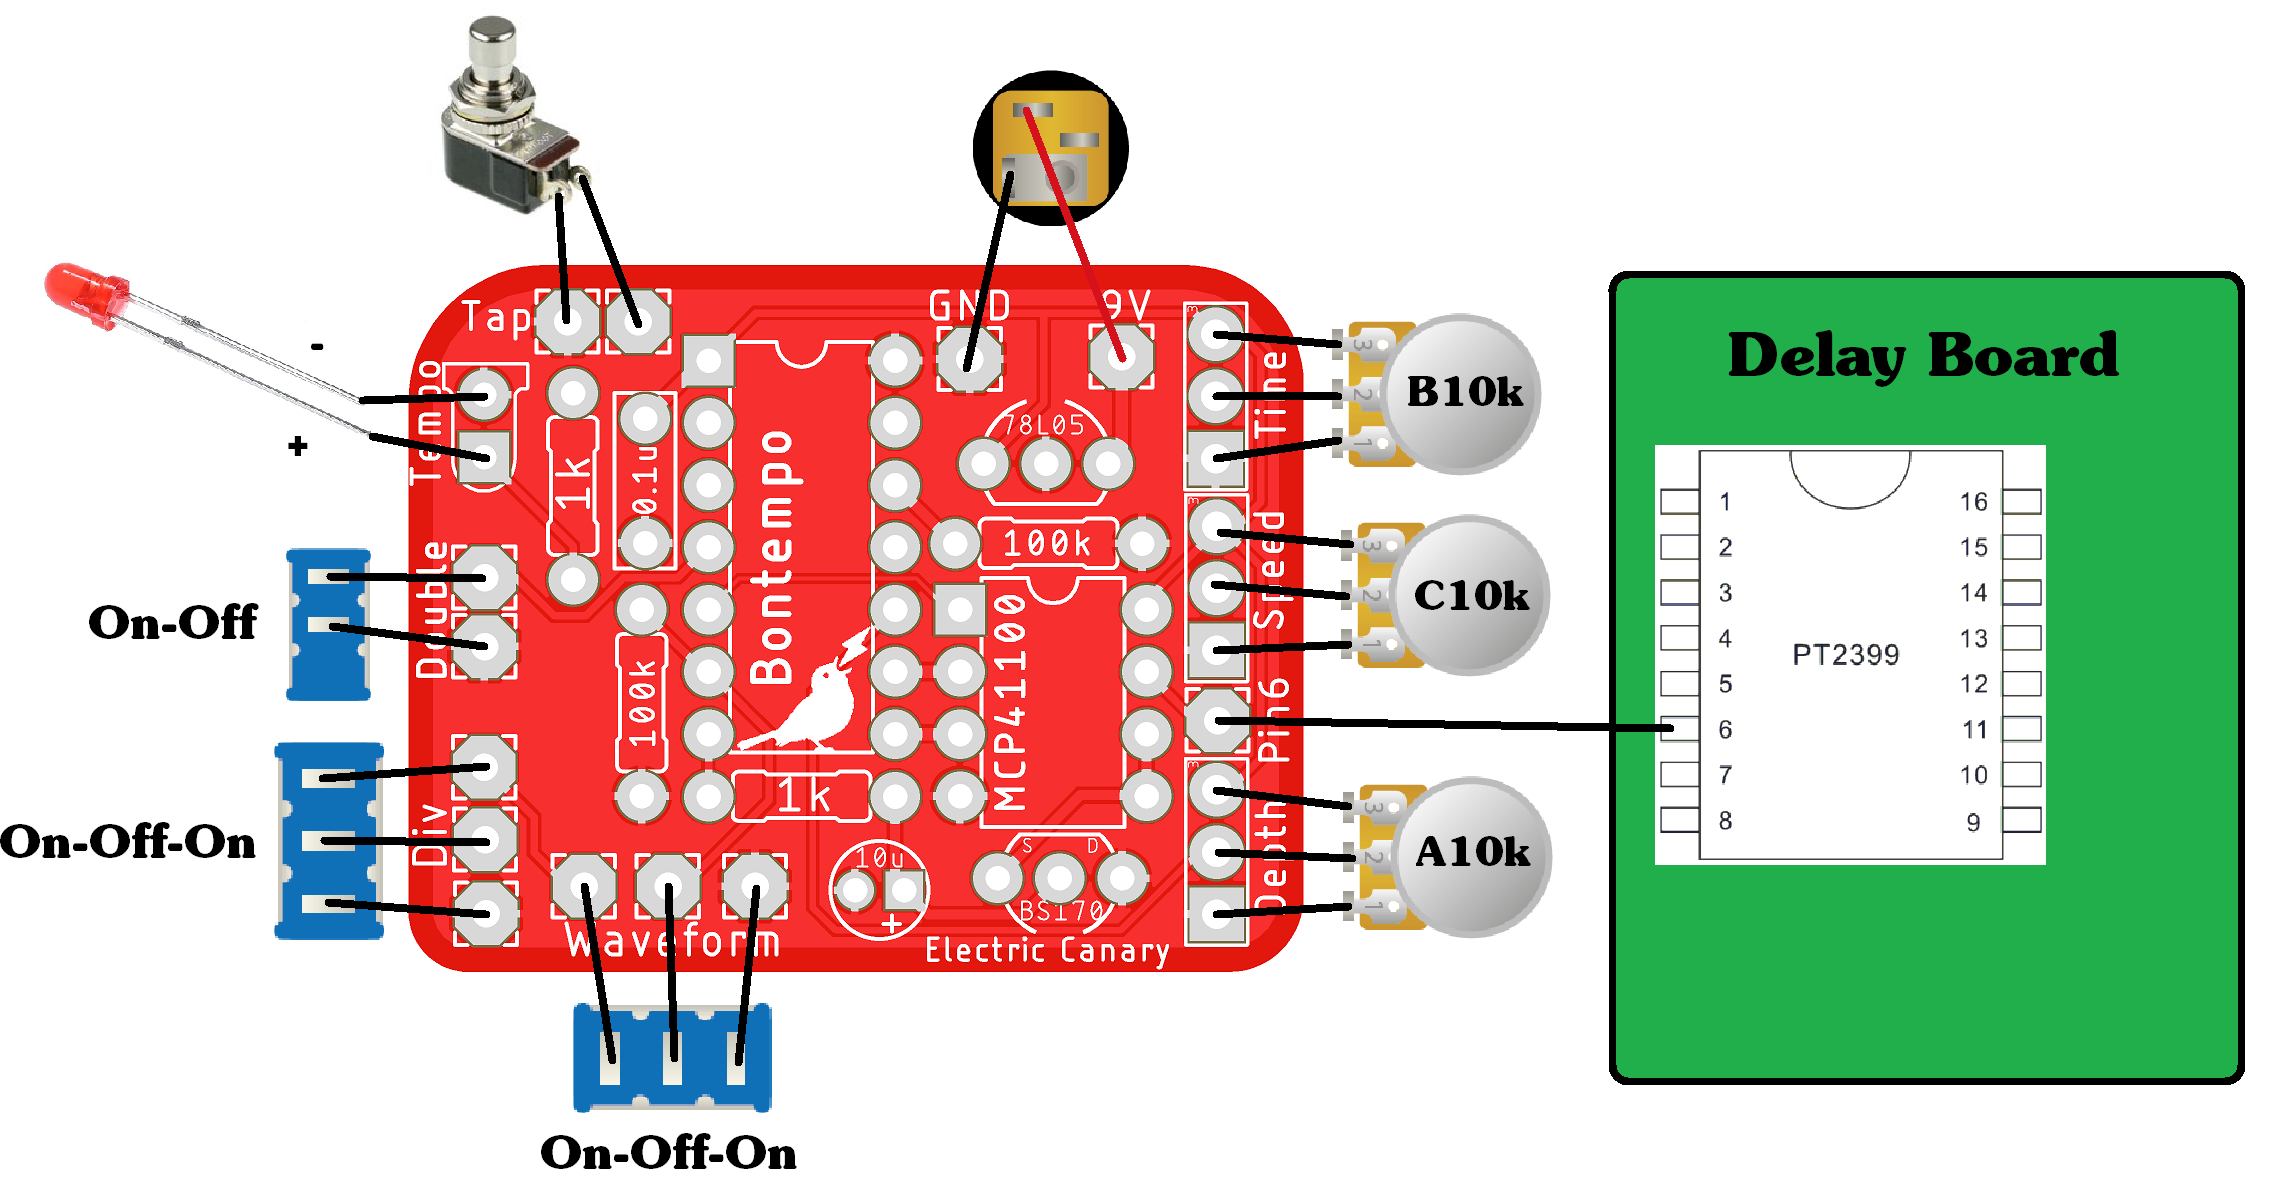
\includegraphics[scale=0.35]{BontempoPCBConnections}
\end{center}
\section{Build Notes}
\begin{itemize}
\item Don't forget to calibrate the Tap Tempo once you're finished ! (\href{https://electric-canary.com/assets/bontempo---datasheet.pdf}{\underline{Datasheet}} Section 9.)
\item Make sure to omit the Delay Time Pot and any resistors connected to the PT2399 Pin6 in the delay circuit. 
\item Make sure the connection between the Bontempo Board and the Delay Board is as short and secured as possible. 
\item If you don't wish to use the Double Time switch dynamically just omit the switch.
\item Theoretically any value between 5k$\Omega$ and 140k$\Omega$ could work for R3 and R4.
\item Similarly, higher values for the pots could be used. Lower values are not recommended.
\item If the LED is too bright you can augment R1 value. 4.7k$\Omega$ can be nicer for super-bright LEDs.
\item Square pads represent pin 1 of pots, + for LED, + for polarized capacitors and pin 1 for ICs.
\item Mind the way you orient switches.
\end{itemize}
\end{document}